\documentclass{article}
\usepackage{tikz}
\usepackage{amsmath}
\usepackage{graphicx}
\usepackage[utf8]{inputenc}
\usepackage{amssymb}
\usepackage{geometry}
\usepackage{fancyhdr}
\usepackage{hyperref}
\usepackage{listings}
\usepackage{color}
\usepackage{ctex}
% \usepackage{subfigure}
\usepackage{subcaption}
\usepackage{float}
\usepackage{amssymb}
\usepackage{amsthm}
\usepackage{algorithm}
\usepackage{algorithmic}
\usepackage{caption}
\usepackage{bm}
\definecolor{dkgreen}{rgb}{0,0.6,0}
\definecolor{gray}{rgb}{0.5,0.5,0.5}
\definecolor{mauve}{rgb}{0.58,0,0.82}
\lstset{
  frame=tb,
  language=Matlab,
  aboveskip=3mm,
  belowskip=3mm,
  showstringspaces=false,
  columns=flexible,
  basicstyle={\small\ttfamily},
  numbers=left,
  numberstyle=\tiny\color{gray},
  keywordstyle=\color{blue},
  commentstyle=\color{dkgreen},
  stringstyle=\color{mauve},
  breaklines=true,
  breakatwhitespace=true,
  tabsize=3
}
\usetikzlibrary{math}
\usetikzlibrary{shapes.geometric, arrows}
\usetikzlibrary{matrix}
\tikzstyle{block} = [draw, rectangle, minimum height=2em, minimum width=4em]
\tikzstyle{sum} = [draw, circle, node distance=1cm]
\tikzstyle{input} = [coordinate]
\tikzstyle{output} = [coordinate]
\tikzstyle{pinstyle} = [pin edge={to-,thin,black}]

\begin{document}
\section*{系统建模问题背景}
\subsection*{问题 4}

试用 Simulink 搭建如下倒立摆的 PID 和 LQR 控制器,假设倒立摆的状态空间模型为:

\begin{align*}
\dot{x} &= Ax+Bu \\
y &= Cx+Du=\left[\begin{matrix}
    \theta\\x
\end{matrix}\right]
\end{align*}

状态矩阵\(A=\left[\begin{matrix}
    0&1&0&0\\41.63&0&0&0\\0&0&0&1\\-0.6099&0&0&0
\end{matrix}\right]\),\(B=\left[\begin{matrix}
    0\\-2.7584\\0\\0.6898
\end{matrix}\right]\),\(C=\left[\begin{matrix}
    1&0&0&0\\0&0&1&0
\end{matrix}\right]\),\(D=\left[\begin{matrix}
    0\\0
\end{matrix}\right]\),状态向量 \( x(t) = \begin{bmatrix} \theta \\ \dot{\theta} \\ x \\\dot{x} \end{bmatrix} \),控制输入 \( u(t) \),输出 \( y(t) \)。

\begin{center}
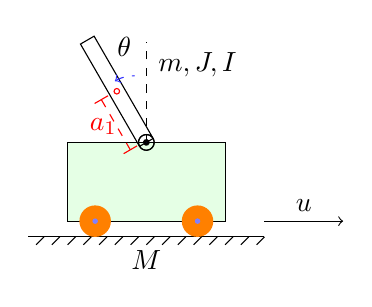
\begin{tikzpicture}
%%%% floor 
%%%%%%  circle of pole 
\tikzmath{ 
\a = sin(30); 
\b = cos(30); 
\bb = -\b+0.2; 
\lp=-1.5; 
\rp=1.5; 
\cartleft=1; 
\cartoff1=0.2; 
} 
\draw (\lp,0) to (\rp,0); 
\foreach \x in {1,...,15} { 
    \coordinate (m\x) at (0.2*\x+\lp,0); 
    \coordinate (n\x) at (0.2*\x+\lp-0.1,-0.1); 
    \draw (m\x) to (n\x); 
} 
\pgfmathsetmacro{\offset}{0.35} 
\pgfmathsetmacro{\lrp}{-\cartleft+\offset} 
\pgfmathsetmacro{\rrp}{\cartleft-\offset} 
\pgfmathsetmacro{\radi}{\cartoff1} 
%%%%%% cart 
\pgfmathsetmacro{\cartheight}{1} 
\pgfmathsetmacro{\cartcriclep}{-1.5} 
\def\rectanglepath{-- ++(2cm,0cm) -- ++(0cm,\cartheight cm) -- ++(-2cm,0cm) -- cycle} 
\fill[opacity=0.5,green!20!white] (-\cartleft,\radi) \rectanglepath; 
\draw (-\cartleft,\radi) \rectanglepath; 
%%%%%%  wheel 1 and wheel 2 
\fill[orange] (\lrp,\radi) circle [radius=\radi cm]; 
\fill[blue!50] (canvas cs:x=\lrp cm,y=\radi cm) circle (1pt); 
\fill[orange] (\rrp,\radi) circle [radius=\radi cm]; 
\fill[blue!50] (canvas cs:x=\rrp cm,y=\radi cm) circle (1pt); 
%%%%%%  circle on the cart 
\pgfmathsetmacro{\raditop}{\radi+1} 
\draw (0,\raditop) circle [radius=0.5*\radi cm]; 
%%%%%%   pole 1 
\pgfmathsetmacro{\polepoint}{1.5} 
\pgfmathsetmacro{\poleheight}{\raditop} 
\def\recpole1{rectangle ++(0.2cm,1.5cm)}; 
\pgfmathsetmacro{\angl}{30} 
\pgfmathsetmacro{\angml}{90+\angl} 
\draw[yshift=\poleheight cm,rotate=\angl] (-0.1,0) \recpole1 (\angml:0 cm) coordinate (P1) circle [radius=0.5*\radi cm] (\angml:0 cm) coordinate (P2) circle (1pt); 
\fill (canvas cs:x=0cm,y=\raditop cm) circle (1pt); 
%%%%% angle note 
\coordinate (point1) at (0cm,\raditop); 
\coordinate (point2) at (P1); 
\tikzmath{ 
\pos3=\raditop+0.85*\polepoint; 
\pos1=\raditop+0.6*\polepoint*\b; 
\pos2=\raditop+\polepoint; 
} 
\tikzmath{ 
\l=cos(90-25); 
\pos1=\raditop+0.6*\polepoint*\b; 
\pos2=\raditop+\polepoint; 
} 
%%%% angle 1 
\draw[red] (point1)++(\angml:0.5*\polepoint cm) coordinate (m1) circle (1pt); 
%%%% L 
\draw[transform canvas={xshift=-0.2cm,yshift=-0.1cm},red,dashed,|-|](m1)--(point1) [xshift=-0.05cm,yshift=0.3cm] node[left=0.0pt] {$a_1$}; 
\path [draw,dashed] (point1)--(point2) [draw,blue!80,<-] (-\a+0.1 ,\pos1) arc(\angml:90:0.5cm); 
\draw[dashed,black] (point1)--++(0cm,0.4*\pos3) node[right=0.8pt] {$m,J,I$} -- (0cm,\pos3) ; 
%%%% theta 
\path (point1) ++(103:1.25cm) node{$\theta$} ; 
%%%% mass M 
\node at (0,\radi-0.5) {$M$}; 
%%%% arrow ->u 
\draw[->] (1.5,\radi) -- (2.5,\radi) node[midway, above] {$u$}; 
%\fill[ultra nearly opaque] 
\end{tikzpicture}
\end{center}

其中,$M$为摆杆的质量,$m$为小球的质量,$J$为摆杆的转动惯量,
$I$为小球的质量矩(这里两种模型的$J,I$可以看为一种东西),$u$为输入力,
$\theta$为摆杆与水平线的夹角,$l$为摆杆重心与水平线的距离。
这里给出假设: $M=1.42,m=0.12,b=0.1,l=0.188,J=I=0.0014$,均为国际单位制(kg,m,s)。
\section*{数学推导与模型构建}
如下图所示,我们拥有两种倒立摆系统的模型假设:
\begin{itemize}
    \item 在杆模型中,我们假设杆的质量是均匀分布的,并且不考虑系统的摩擦。
    \item 在球模型中,我们胡烈摆杆质量和地面摩擦,并且假设杆的质量集中在杆的末端。
\end{itemize}
这种假设影响的是重心位置,但是我们可以通过巧妙地让重心到连接点的长度为$l$来寻找统一的表达式。
\begin{figure}[htbp]
    \centering
    \begin{subfigure}[b]{0.45\textwidth}
        \centering
        \includegraphics[width=\textwidth]{imgs/figure1.png}
        \caption{倒立摆杆质量模型}
        \label{fig:杆质量模型}
    \end{subfigure}
    \hfill
    \begin{subfigure}[b]{0.45\textwidth}
        \centering
        \includegraphics[width=\textwidth]{imgs/figure2.png}
        \caption{倒立摆球质量模型}
        \label{fig:球质量模型}
    \end{subfigure}
    \caption{两种倒立摆模型}
    \label{fig:两种倒立摆模型}
\end{figure}
\subsection*{倒立摆杆质量模型}
严格来说:假设$u$为外部作用力,$M$为小车质量, $m$为摆杆质量,
摆杆长度为 $2l$且摆杆质量均匀分布。设 $x$为小车位置, 
$ \theta$ 为摆杆与竖直方向的夹角。系统不考虑空气阻力的影响。
那么我们根据牛顿第二定律,考虑摆杆重心的水平运动和垂直运动,然后在考虑小车的水平运动和摆杆的转动(绕重心的转动运动)。
\[
\left\{\begin{matrix}
    m\frac{d^2}{dt^2}(x+l\sin(\theta)) = H \\
    m\frac{d^2}{dt^2}(l\cos(\theta)) = -mg + V \\
    M\frac{d^2}{dt^2}(x) = u - H \\
    I\frac{d^2}{dt^2}(\theta) = Vl\sin(\theta) - Hl\cos(\theta)
\end{matrix}\right.
\]
联立化简即可,我们为了方便后续设计,假设倒立摆角度很小,近似认为\(\sin\theta=\theta,\cos\theta=1\);以及倒立摆绕重心的转动惯量很小,近似认为\(I=0\)。
那么可以得到:
\[
\left\{
    \begin{matrix}
        (M+m)\ddot{x} + ml\ddot{\theta} = u \\
        ml^2\ddot{\theta} + ml\ddot{x} = mgl\theta \\
    \end{matrix}
\right.
\]
定义状态变量$X$:
\[
X = \begin{bmatrix}
    x_1\\x_2\\x_3\\x_4
\end{bmatrix} = \begin{bmatrix}
    \theta \\ \dot{\theta}\\x \\ \dot{x} \\ 
\end{bmatrix}
\]
那么可以得到状态方程:
\[
\dot{X} = \begin{bmatrix}
    \dot{\theta} \\ \dot{\dot{\theta}}\\ \dot{x} \\ \dot{\dot{x}} \\ 
\end{bmatrix} = \begin{bmatrix} x_2\\\frac{(M+m)g}{Ml}x_1-\frac{1}{Ml}u\\x_4\\-\frac{mg}{M}x_1+\frac{1}{M}u \end{bmatrix}
\]
可以写出以为倒立摆系统的状态空间方程表达式:
\[
\begin{bmatrix}
\dot{x_1}\\\dot{x_2}\\\dot{x_3}\\\dot{x_4}    
\end{bmatrix}
=
\begin{bmatrix}
0&1&0&0\\
\frac{(M+m)g}{Ml}&0&0&0\\
0&0&0&1\\
-\frac{mg}{M}&0&0&0
\end{bmatrix}\cdot
\begin{bmatrix}
    x_1\\x_2\\x_3\\x_4
\end{bmatrix} + 
\begin{bmatrix}
0\\
-\frac{1}{Ml}\\
0\\
\frac{1}{M}
\end{bmatrix}\cdot u 
\]

\[
y=CX+D\hat{u}=\begin{bmatrix}
    1&0&0&0\\
    0&0&1&0
\end{bmatrix} \cdot
\begin{bmatrix}
    x_1\\x_2\\x_3\\x_4
\end{bmatrix}+\begin{bmatrix}
    0\\0
\end{bmatrix}\cdot \hat{u}=
\begin{bmatrix}
   \theta \\ x
\end{bmatrix}
\]

\subsection*{倒立摆球质量模型}
严格来说:假设$u$为外部作用力,$M$为小车质量, $m$为摆杆末端球质量,
摆杆长度为 $l$且摆杆质量集中在杆的末端。设 $x$为小车位置, 
$ \theta$ 为摆杆与竖直方向的夹角。系统不考虑空气阻力的影响。

同上述过程,我们考虑倒立摆摆杆重心的水平-垂直运动与小车水平运动和摆杆转动:
\[
\left\{\begin{matrix}
    m\frac{d^2}{dt^2}(x+l\sin(\theta)) = H \\
    m\frac{d^2}{dt^2}(l\cos(\theta)) = -mg + V \\
    M\frac{d^2}{dt^2}(x) = u - H \\
    I\frac{d^2}{dt^2}(\theta) = Vl\sin(\theta) - Hl\cos(\theta)
\end{matrix}\right.
\]
整理一下:
\[\left\{\begin{matrix}
    (M+m)\ddot{x}+ml\ddot{\theta}\cos\theta -ml\dot{\theta}^2\sin\theta = u \\
    ml\ddot{x}\cos\theta+(I+ml^2)\ddot{\theta}-mgl\sin\theta = 0 \\
\end{matrix}
\right.\]

那么我们同样假设在系统平衡点附近,摆杆的角度、角速度可以忽略不计,
即 $\cos\theta=1,\sin\theta=\theta;\dot{\theta} = 0$,
$\sin\theta\dot{\theta} = 0$,则:
\[
\left\{\begin{matrix}
    (M+m)\ddot{x}+ml\ddot{\theta} = u \\
    ml\ddot{x}+(I+ml^2)\ddot{\theta} = mgl\theta \\
\end{matrix}
\right.
\]
定义状态变量$X$:
\[
X = \begin{bmatrix}
    x_1\\x_2\\x_3\\x_4
\end{bmatrix} = \begin{bmatrix}
    \theta \\ \dot{\theta}\\x \\ \dot{x} \\ 
\end{bmatrix}
\]
那么同理我们可以得到系统状态空间方程:
\[
\begin{bmatrix}
\dot{x_1}\\\dot{x_2}\\\dot{x_3}\\\dot{x_4}    
\end{bmatrix}
=
\begin{bmatrix}
0&1&0&0\\
\frac{mgl(M+m)}{I(M+m)+Mml^2}&0&0&0\\
0&0&0&1\\
-\frac{m^2gl^2}{I(M+m)+Mml^2}&0&0&0
\end{bmatrix}\cdot
\begin{bmatrix}
    x_1\\x_2\\x_3\\x_4
\end{bmatrix} + 
\begin{bmatrix}
0\\
-\frac{ml}{I(M+m)+Mml^2}\\
0\\
\frac{I+ml^2}{I(M+m)+Mml^2}
\end{bmatrix}\cdot u 
\]

\[
y=CX+D\hat{u}=\begin{bmatrix}
    1&0&0&0\\
    0&0&1&0
\end{bmatrix} \cdot
\begin{bmatrix}
    x_1\\x_2\\x_3\\x_4
\end{bmatrix}+\begin{bmatrix}
    0\\0
\end{bmatrix}\cdot \hat{u}=
\begin{bmatrix}
   \theta \\ x
\end{bmatrix}
\]
\subsection*{更一般的形式}
我们这里还要考虑近来阻尼系数$b$,那么我们现在的方程就变成了:
\[
\left\{\begin{matrix}
    (M+m)\ddot{x}+b\dot{x}+ml\ddot{\theta} = u \\
    ml\ddot{x}+(I+ml^2)\ddot{\theta} = mgl\theta \\
\end{matrix}
\right.
\]

那么在添加了阻尼系数之后,我们更一般的表达式应该是:
\[
\begin{bmatrix}
\dot{x_1}\\\dot{x_2}\\\dot{x_3}\\\dot{x_4}    
\end{bmatrix}
=
\begin{bmatrix}
0&1&0&0\\
\frac{mgl(M+m)}{p}&-\frac{(I+ml^2)b}{p}&0&0\\
0&0&0&1\\
-\frac{m^2gl^2}{p}&-\frac{mlb}{p}&0&0
\end{bmatrix}\cdot
\begin{bmatrix}
    x_1\\x_2\\x_3\\x_4
\end{bmatrix} + 
\begin{bmatrix}
0\\
-\frac{ml}{p}\\
0\\
\frac{I+ml^2}{p}
\end{bmatrix}\cdot u 
\]

\[
y=CX+D\hat{u}=\begin{bmatrix}
    1&0&0&0\\
    0&0&1&0
\end{bmatrix} \cdot
\begin{bmatrix}
    x_1\\x_2\\x_3\\x_4
\end{bmatrix}+\begin{bmatrix}
    0\\0
\end{bmatrix}\cdot \hat{u}=
\begin{bmatrix}
   \theta \\ x
\end{bmatrix}
\]

其中,$p=I(M+m)+Mml^2$,当然还有$q=(M+m)(I+ml^2)-(ml)^2$,在后面pid调节的时候可以使用。
\section*{控制环节}
\subsection*{LQR控制}
已知系统状态空间模型:
\[
\dot{X}=AX+Bu
\]
其中$X$为状态向量,$u$为控制输入,$A$为状态矩阵,$B$为输入矩阵。

LQR控制考虑最佳控制向量的矩阵$K$:
\[
\hat{u}=u-KX
\]
其中$K$为增益矩阵,$X$为状态向量。

那么LQR控制的目标转换为确定下列最小化二次型函数:
\[
J=\frac{1}{2}\int_{0}^{T}(X^TQX+u^TRu)dt
\]
此时不妨选择$Q=I,R=I$,使用matlab代码求解得到增益矩阵$K$:
\begin{lstlisting}[language=matlab,numbers=none]
% 倒立摆系统参数
M = 1.42;     % 小车质量
m = 0.12;     % 摆球质量
l = 0.188;    % 摆杆长度
I = 0.0014;     % 摆球转动惯量
g = 9.8;      % 重力加速度9.8m/s^2
q = (M+m)*(I+m*l^2)-(m*l)^2;
p = I*(M+m)+(M*m*l^2);
% 倒立摆系统状态空间矩阵定义
A = [0               1 0 0
    (M+m)*m*g*l/(I*(M+m)+(M*m*l^2))    0 0 0
    0                0 0 1
    -m^2*g*l^2 /(I*(M+m)+(M*m*l^2))          0 0 0];
B = [0 -m*l/(I*(M+m)+(M*m*l^2)) 0 (I+m*l^2)/(I*(M+m)+(M*m*l^2))]';
Q=eye(4);
R=eye(1);
K=lqr(A,B,Q,R);
\end{lstlisting}
此时可以输出得到$k=[-36.9690   ,-5.8463   ,-1.0000   ,-2.3376]$。

那么我们拥有了这个k,就可以搭建LQR控制器了,首先考虑如下理论模型,我们注意到,
在LQR控制器中,反馈K到输入u中,然后在乘以B,与A反馈相加之后。
\begin{figure}[htbp]
    \centering
    \includegraphics[width=0.95\textwidth]{./imgs/LQR_OPTi.png}
    \caption{LQR控制器}
\end{figure}

\subsection*{PID控制}
进行laplace变换,同时假设$\theta,\dot{\theta}$很小,根据上述推导不难有如下式子:
\[\left\{\begin{matrix}
    (M+m)\ddot{x}+ml\ddot{\theta}\cos\theta -ml\dot{\theta}^2\sin\theta + b\dot{x} = u \\
    ml\ddot{x}\cos\theta+(I+ml^2)\ddot{\theta}-mgl\sin\theta = 0 \\
\end{matrix}
\right.\]

有初始状态为0,而且$\sin\theta=\theta,\cos\theta=1,\dot{\theta}=0$:

\[
(I+ml^2)\Phi(s)s^2-mgl\Phi(s)=mlX(s)s^2-ml\Phi(s)s^2+bX(s)s=U(s)
\]

那么可以给出两种传递函数:
\[
P_\text{pend}(s)=\frac{\Phi(s)}{U(s)}=\frac{mls}{((M+m)(I+ml^2)-(ml)^2)s^3+b(I+ml^2)s^2-(M+m)mgls-bmgl}
\]
\[
P_\text{cart}(s)=\frac{X(s)}{U(s)}=\frac{(I+ml^2)s^2-mgl}{((M+m)(I+ml^2)-(ml^2))s^4+b(I+ml^2)s^3-(M+m)mgls^2-bmgls}
\]

当然,我们还有另外一种传递函数:
\[
\left\{
    \begin{matrix}
    \ddot{x}=\frac{(I+ml^2)u+ml(I+ml^2)\dot{\theta}^2\sin\theta-m^2l^2g\sin\theta\cos\theta}{(I+ml^2)(M+m)-m^2l^2\cos^2\theta}\\
    \ddot{\theta}=\frac{mlu\cos\theta+m^2l^2\dot{\theta}^2\sin\theta\cos\theta-(M+m)mlg\sin\theta}{m^2l^2\cos^2\theta-(I+ml^2)(M+m)}
    \end{matrix}
\right.
\]
这个时候带入$\theta\to 0$求解,有:
\[
\left\{
    \begin{matrix}
    \ddot{x}=\frac{0.0022u-0.005\theta}{0.0082}\\
    \ddot{\theta}=\frac{0.0226u-0.3405\theta}{-0.0082}
    \end{matrix}
\right.
\]
所以在平衡点附近的参数就线性化为:
\[
\left\{
    \begin{matrix}
    \ddot{x}=0.2683u-0.6098\theta\\
    \ddot{\theta}=-2.7561u+41.5244\theta
    \end{matrix}
\right.
\]
然后laplace变换,得到:
\[
\left\{
    \begin{matrix}
    X(s)=\frac{-0.0973s^2+3.4325}{s^2}\Phi(s)\\
    \Phi(s)=\frac{-2.7561}{s^2-41.5244}U(s)
    \end{matrix}
\right.
\]
我们根据这个可以画出来系统框图如下:
\begin{center}
    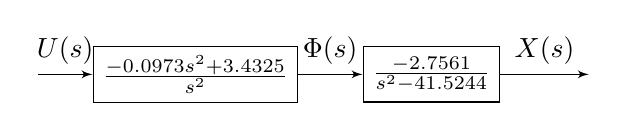
\begin{tikzpicture}[auto, node distance=2cm, >=latex']
        % 定义输入节点
        \node [input, name=input] {};
        % 定义第一个传递函数
        \node [block, right of=input] (G1) {$\frac{-0.0973s^2 + 3.4325}{s^2}$};
        % 定义第二个传递函数
        \node [block, right of=G1, node distance=3cm] (G2) {$\frac{-2.7561}{s^2 - 41.5244}$};
        % 定义输出节点
        \node [output, right of=G2] (output) {};
        % 连接各个节点
        \draw [->] (input) -- node {$U(s)$} (G1);
        \draw [->] (G1) -- node {$\Phi(s)$} (G2);
        \draw [->] (G2) -- node [name=X] {$X(s)$} (output);
        % 添加反馈路径
        % \draw [->] (G2.south) -- ++(0,-1.5cm) -| node [pos=0.99] {$-$} (G1.south);
    \end{tikzpicture}
\end{center}
这样关于角度和关于小车位移的传递函数就有了,可以进行pid控制仿真了。
\begin{lstlisting}[language=matlab,numbers=none]
%Modeling
%%Transfer Function
mCart = 1.42;  
mPend = 0.12;
b = 0.1;     % 阻尼系数
I = 0.014;     % 转动惯量
g = 9.8;
L = 0.188;
q = (mCart+mPend)*(I+mPend*L^2)-(mPend*L)^2;
s = tf('s');
P_cart = (((I+mPend*L^2)/q)*s^2 - (mPend*g*L/q))/(s^4 + (b*(I + mPend*L^2))*s^3/q - ((mCart + mPend)*mPend*g*L)*s^2/q - b*mPend*g*L*s/q);
P_pend = (mPend*L*s/q)/(s^3 + (b*(I + mPend*L^2))*s^2/q - ((mCart + mPend)*mPend*g*L)*s/q - b*mPend*g*L/q);
sys_tf = [P_cart ; P_pend]
inputs = {'u'};
outputs = {'x'; 'phi'};
set(sys_tf,'InputName',inputs)
set(sys_tf,'OutputName',outputs)
% PID环节
Kp = 100;
Ki = 1;
Kd = 30;
C = pid(Kp,Ki,Kd);
T1 = feedback(P_pend,C);
T2 = feedback(1,P_pend*C)*P_cart;
\end{lstlisting}

我们现在有输出如下:
\[
\begin{matrix}
P_\text{cart} =\frac{1.388 \times 10^{-5} s^2 - 0.0001682}{2.098 \times 10^{-5} s^4 + 1.388 \times 10^{-6} s^3 - 0.000259 s^2 - 1.682 \times 10^{-5} s} & \text{从输入U(s)到输出1X(s)} \\
P_\text{pend} =\frac{1.716 \times 10^{-5} s}{2.098 \times 10^{-5} s^3 + 1.388 \times 10^{-6} s^2 - 0.000259 s - 1.682 \times 10^{-5}} & \text{从输入U(s)到输出2}\Phi(S)
\end{matrix}
\]

随后我们转化:
\[
\begin{matrix}
\text{T1} =
\frac{1.716 \times 10^{-5} s^2}{2.098 \times 10^{-5} s^4 + 0.0005163 s^3 + 0.001457 s^2 + 3.433 \times 10^{-7} s}
\\
\text{T2} =
\frac{2.912 \times 10^{-10} s^6 + 1.926 \times 10^{-11} s^5 - 7.125 \times 10^{-9} s^4 - 4.669 \times 10^{-10} s^3 + 4.357 \times 10^{-8} s^2 + 2.829 \times 10^{-9} s}{4.404 \times 10^{-10} s^8 + 1.086 \times 10^{-8} s^7 + 2.586 \times 10^{-8} s^6 - 1.321 \times 10^{-7} s^5 - 3.862 \times 10^{-7} s^4 - 2.46 \times 10^{-8} s^3 - 5.774 \times 10^{-12} s^2}
\end{matrix}
\]
这个时候我们可以直接运算T1,T2的脉冲响应即可。

而同时我们也有这样的PID控制器框图如下:
\begin{figure}[htbp]
    \centering
    \includegraphics[width=0.95\textwidth]{./imgs/PID_OPTi.png}
    \caption{双PID控制器}
\end{figure}
\section*{Matlab代码与Simulink仿真测试}
\subsection*{LQR控制}
根据上述操作,我们已经大概知道了怎么计算,现在我们进行matlab仿真测试。
\begin{lstlisting}[language=matlab,numbers=none]
% 倒立摆系统参数
M = 1.42;     % 小车质量
m = 0.12;     % 摆球质量
l = 0.188;    % 摆杆长度
I = 0.0014;     % 摆球转动惯量
g = 9.8;      % 重力加速度9.8m/s^2
q = (M+m)*(I+m*l^2)-(m*l)^2;
p = I*(M+m)+(M*m*l^2);
% 倒立摆系统状态空间矩阵定义
A = [0               1 0 0
    (M+m)*m*g*l/(I*(M+m)+(M*m*l^2))    0 0 0
    0                0 0 1
    -m^2*g*l^2 /(I*(M+m)+(M*m*l^2))          0 0 0];
B = [0 -m*l/(I*(M+m)+(M*m*l^2)) 0 (I+m*l^2)/(I*(M+m)+(M*m*l^2))]';
C = [1 0 0 0
    0 0 1 0];
D = 0;
% 倒立摆系统状态空间模型
G = ss(A, B, C, D)
\end{lstlisting}
我们有输出如下,可以看出,尽管我们定义了阻尼系数b,
但是这道题这样给出来的状态矩阵就是没有计算阻尼系数的形式,但是与题目所给形式完全一致:
\begin{lstlisting}[numbers=none]
G =
  A = 
            x1       x2       x3       x4
   x1        0        1        0        0
   x2    41.63        0        0        0
   x3        0        0        0        1
   x4  -0.6099        0        0        0
  B = 
           u1
   x1       0
   x2  -2.758
   x3       0
   x4  0.6898
  C = 
      x1  x2  x3  x4
   y1   1   0   0   0
   y2   0   0   1   0
  D = 
       u1
   y1   0 
   y2   0
连续时间状态空间模型。
\end{lstlisting}
那么根据之前讨论过的(主要参考控制环节-LQR控制),这里主要使用了图2中的理论系统形式,我们可以搭出LQR控制器的simulink文件:
\begin{figure}[htbp]
    \centering
    \includegraphics[width=0.95\textwidth]{imgs/simulink_lqr.png}
    \caption{simulink仿真文件}    
\end{figure}
\subsubsection*{完整代码}
\begin{lstlisting}[language=matlab,numbers=none]
% 定义状态矩阵 A 和控制矩阵 B 观测矩阵 C 和输入矩阵 D
A = [0, 1, 0, 0;
     41.63, 0, 0, 0;
     0, 0, 0, 1;
     -0.6099, 0, 0, 0];
B = [0;
     -2.7584;
     0;
     0.6898];
C = [1, 0, 0, 0;
     0, 0, 1, 0];
D = [0;
     0];
G = ss(A, B, C, D);
% 定义权重矩阵 Q 和 R
Q = eye(4);  % 状态权重矩阵,这里使用单位矩阵
R = 1;       % 控制权重矩阵,这里使用 1
[K, S, E] = lqr(A, B, Q, R);
B
A
K
A_cl = A - B * K;
B_cl = B;
C_cl = C;
D_cl = D;
Gclose = ss(A_cl, B_cl, C_cl, D_cl);

% 计算并绘制阶跃响应
t = 0:0.01:10;
[y, t, x] = step(Gclose, t);

figure;
% 摆角与角速度响应
subplot(2, 1, 1);
plot(t, x(:, 1), 'b-', 'LineWidth', 2);
hold on;
plot(t, x(:, 2), 'r--', 'LineWidth', 2);
grid on;
xlabel('time(s)', 'FontSize', 20);
ylabel('{\theta and \dot \theta}', 'FontSize', 20);
title('摆角与角速度响应', 'FontSize', 25);
legend('摆角', '角速度');
% 位移与速度响应
subplot(2, 1, 2);
plot(t, x(:, 3), 'g-', 'LineWidth', 2);
hold on;
plot(t, x(:, 4), 'm--', 'LineWidth', 2);
grid on;
xlabel('time(s)', 'FontSize', 20);
ylabel('{x and \dot x}', 'FontSize', 20);
title('位移与速度响应', 'FontSize', 25);
legend('位移', '速度');

set(gcf, 'Position', [100, 100, 800, 600]);
\end{lstlisting}
\subsection*{PID控制}
那么根据之前讨论过的(主要参考),我们可以搭出PID控制器的simulink文件:
\begin{figure}[htbp]
    \centering
    \includegraphics[width=0.95\textwidth]{imgs/simulink_pid.png}
    \caption{simulink仿真文件}    
\end{figure}
\subsubsection*{完整代码}
\begin{lstlisting}[language=matlab,numbers=none]
%Modeling
%%Transfer Function
mCart = 1.42;  
mPend = 0.12;
b = 0.1;     % 阻尼系数
I = 0.014;     % 转动惯量
g = 9.8;
L = 0.188;
q = (mCart+mPend)*(I+mPend*L^2)-(mPend*L)^2;
s = tf('s');
P_cart = (((I+mPend*L^2)/q)*s^2 - (mPend*g*L/q))/(s^4 + (b*(I + mPend*L^2))*s^3/q - ((mCart + mPend)*mPend*g*L)*s^2/q - b*mPend*g*L*s/q);
P_pend = (mPend*L*s/q)/(s^3 + (b*(I + mPend*L^2))*s^2/q - ((mCart + mPend)*mPend*g*L)*s/q - b*mPend*g*L/q);
sys_tf = [P_cart ; P_pend]
inputs = {'u'};
outputs = {'x'; 'phi'};
set(sys_tf,'InputName',inputs)
set(sys_tf,'OutputName',outputs)
t = 0:0.05:5;
u = ones(size(t));
[y,t] = lsim(sys_tf,u,t);
figure ;
plot(t,y) ;
title('Open-Loop Step Response') ;
% axis([0 3 0 50]) ;
legend('x','phi');
% PID环节
Kp = 100;
Ki = 1;
Kd = 30;
C = pid(Kp,Ki,Kd);
T1 = feedback(P_pend,C);
t=0:0.01:4;
figure;
subplot(2,1,1);
impulse(T1,t)
title('Close-loop impluse Response')
legend('phi');
% figure;
T2 = feedback(1,P_pend*C)*P_cart;
t = 0:0.01:5;
subplot(2,1,2);
impulse(T2, t);
title('Close-loop impluse Response')
legend('x');
\end{lstlisting}
\end{document}



%%%%% Not used , but very cool , so i keep that in this code:
% \begin{center}
% \begin{tikzpicture}
% %%%% floor 
% %%%%%%  circle of pole 
% \tikzmath{ 
% \a = sin(30); 
% \b = cos(30); 
% \bb = -\b+0.2; 
% \lp=-1.5; 
% \rp=1.5; 
% \cartleft=1; 
% \cartoff1=0.2; 
% %\mycount = log10(2048) / log10(2); 
% %\mydimen = 15^2; 
% } 
% \draw (\lp,0) to (\rp,0); 
% \foreach \x in {1,...,15} { 
%     \coordinate (m\x) at (0.2*\x+\lp,0); 
%     \coordinate (n\x) at (0.2*\x+\lp-0.1,-0.1); 
%     \draw (m\x) to (n\x); 
%       } 
% \pgfmathsetmacro{\offset}{0.35} 
% \pgfmathsetmacro{\lrp}{-\cartleft+\offset} 
% \pgfmathsetmacro{\rrp}{\cartleft-\offset} 
% \pgfmathsetmacro{\radi}{\cartoff1} 
% %%%%%% cart 
% \pgfmathsetmacro{\cartheight}{1} 
% \pgfmathsetmacro{\cartcriclep}{-1.5} 
% \def\rectanglepath{-- ++(2cm,0cm) -- ++(0cm,\cartheight cm) -- ++(-2cm,0cm) -- cycle} 
% \fill[opacity=0.5,green!20!white] (-\cartleft,\radi) \rectanglepath; 
% \draw (-\cartleft,\radi) \rectanglepath; 
% %%%%%%  wheel 1 and wheel 2 
% \fill[orange] (\lrp,\radi) circle [radius=\radi cm]; 
% \fill[blue!50] (canvas cs:x=\lrp cm,y=\radi cm) circle (1pt); 
% \fill[orange] (\rrp,\radi) circle [radius=\radi cm]; 
% \fill[blue!50] (canvas cs:x=\rrp cm,y=\radi cm) circle (1pt); 
% %%%%%%  circle on the cart 
% \pgfmathsetmacro{\raditop}{\radi+1} 
% \draw (0,\raditop) circle [radius=0.5*\radi cm]; 
% %%%%%%   pole 1 and pole 2 
% \pgfmathsetmacro{\polepoint}{1.5} 
% \pgfmathsetmacro{\poleheight}{\raditop} 
% \def\recpole1{rectangle ++(0.2cm,1.5cm)}; 
% \pgfmathsetmacro{\angl}{30} 
% \pgfmathsetmacro{\angu}{25} 
% \pgfmathsetmacro{\angml}{90+\angl} 
% \pgfmathsetmacro{\angmu}{90+\angl+\angu} 
% \draw[yshift=\poleheight cm,rotate=\angl] (-0.1,0) \recpole1 [yshift=\polepoint cm, rotate=\angu](-0.1,0) \recpole1 (\angml:0 cm) coordinate (P1) circle [radius=0.5*\radi cm] (\angml:0 cm) coordinate (P2) circle (1pt); 
% \fill (canvas cs:x=0cm,y=\raditop cm) circle (1pt); 
% %%%%% angle note 
% \coordinate (point1) at (0cm,\raditop); 
% \coordinate (point2) at (P1); 
% \tikzmath{ 
% \pos3=\raditop+0.85*\polepoint; 
% \pos1=\raditop+0.6*\polepoint*\b; 
% \pos2=\raditop+\polepoint; 
% } 
% \tikzmath{ 
% \l=cos(90-25); 
% \pos1=\raditop+0.6*\polepoint*\b; 
% \pos2=\raditop+\polepoint; 
% } 
% %%%% angle 1 
% \draw[red] (point1)++(\angml:0.5*\polepoint cm) coordinate (m1) circle (1pt); 
% %%%% a_1 
% \draw[transform canvas={xshift=-0.2cm,yshift=-0.1cm},red,dashed,|-|](m1)--(point1) [xshift=-0.05cm,yshift=0.3cm] node[left=0.0pt] {$a_1$}; 
% \path [draw,dashed] (point1)--(point2) [draw,blue!80,<-] (-\a+0.1 ,\pos1) arc(\angmu:90:0.5cm); 
% \draw[dashed,blue] (point1)--++(0cm,0.4*\pos3) node[right=0.8pt] {$m_1,I_1,J_1$} -- (0cm,\pos3) ; 
% %%%% angle 2 
% \draw[red] (point2)++(\angmu:0.5*\polepoint cm) coordinate (m2) circle (1pt); 
% %%%% a_2 
% \draw[transform canvas={xshift=-0.2cm,yshift=-0.2cm},red,dashed,|-|](m2)--(point2) [xshift=-0.1cm,yshift=0.05cm] node[left=0.0pt] {$a_2$}; 
% \draw[dashed,blue!50] (point2)-- ++(0,1); 
% \pgfmathsetmacro{\angall}{\angmu} 
% \draw[dashed,blue!70] (point2)-- ++(\angall:\polepoint cm) 
% [draw,blue!70,<-] (point2)-- ++(\angall:0.4*\polepoint cm) node[left=3pt,xshift=-0.2cm] {$m_2,I_2,J_2$} arc(\angall:90:0.5cm); 
% %%%% varphi 1 --- varphi 2 
% \path (point1) ++(103:1.25cm) node{$\varphi_1$} ; 
% \path (point2) ++(110:0.85cm) node{$\varphi_2$}; 
% %\fill[ultra nearly opaque] 
% \end{tikzpicture}
% \end{center}
